\documentclass{beamer}

\usetheme{Berlin}

\makeatother
\setbeamertemplate{footline}
{
  \leavevmode%
  \hbox{%
  \begin{beamercolorbox}[wd=.4\paperwidth,ht=2.25ex,dp=1ex,center]{author in head/foot}%
    \usebeamerfont{author in head/foot}PL22 Grupo 3
  \end{beamercolorbox}%
  \begin{beamercolorbox}[wd=.6\paperwidth,ht=2.25ex,dp=1ex,center]{title in head/foot}%
    \usebeamerfont{title in head/foot}O Pêndulo\hspace*{3em}

  \end{beamercolorbox}}%
  \vskip0pt
}
\makeatletter
\setbeamertemplate{navigation symbols}{}


\usepackage[latin1,utf8]{inputenc} \usepackage[portuguese]{babel}
\usepackage{multicol}
\usepackage{verbatim}
%\usepackage[document]{ragged2e}
\usepackage{tabularx}
\usepackage{adjustbox}
\usepackage{graphicx}
\usepackage{pgfplots} 

\pgfplotsset{width=10cm,compat=1.9}

\title{O Pêndulo \newline Física Experimental I}
\author{Ernesto González 52857 \newline Gonçalo Jesus 52874 \newline Patricia Magalhães 52871 \newline Tiago Pereira 53107}
\date{29 de Abril, 2019}


\begin{document}

\maketitle

\begin{frame}
	\frametitle{O pêndulo simples}
	Um pêndulo simples é um sistema que 		pode oscilar devido à ação 					gravitacional, procurando o estado mais baixo de energia, e que está 		configurado por uma massa pontual 			\textit{m} suspensa de um ponto fixo 		por um fio inextensível e de massa 			desprezável.
	\begin{figure}
		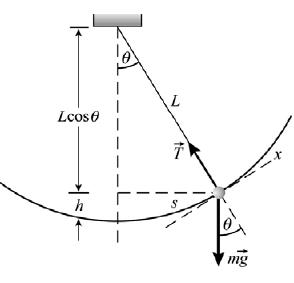
\includegraphics[scale=0.6]{pendulosimples}\caption{Pêndulo simples}
	\end{figure}

\end{frame}

\begin{frame}
	\frametitle{O pêndulo simples }
	Na ausência de atrito, a massa descreve um movimento harmónico simples:
	$$ \theta = \theta _{max} \sin (\omega 	t + \phi _0) $$
	Este tipo de movimentos têm associados 	uma frequência angular, $ \omega $ que 	depende do 				comprimento do fio, $ \ell 	$:
	$$ \omega = \sqrt{\frac{g}{\ell}} \iff T = 2 \pi \sqrt{\frac{\ell}{g}} $$
\end{frame}

\begin{frame}
	\frametitle{O pêndulo físico}
	Um pêndulo físico consiste num corpo rígido suspenso de um ponto fixo. Para pequenas oscilações temos 
	$$ \theta = \theta _{max} \sin (\omega 		t + \phi _0)\quad e \quad T = 2 \pi 			\sqrt{\frac{\mathrm{I}}{mgh}}$$
       \begin{tabular}{cl}  
         \begin{tabular}{c}

  			    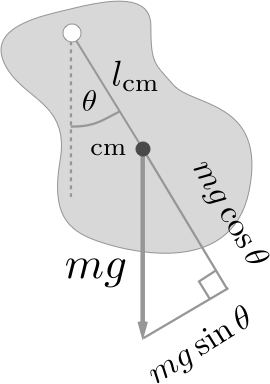
\includegraphics[scale=0.3]{pendulofisico}

 
           \end{tabular}
           & \begin{tabular}{l}
             \parbox{0.5\linewidth}{%  change the parbox width as appropiate
            O estudo das Figura 1 e Figura 2 revela uma importante diferença entre o pêndulo simples e o 					pêndulo físico. Para um pêndulo físico a força restauradora $ F_g \sin \theta $ da força 				gravitacional tem um braço de distância \textit{h} ao ponto pivot, em vez do comprimento 				do fio $ \ell $ .
    		}			
         \end{tabular}  \\
\end{tabular}
\end{frame}

\begin{frame}  
	\frametitle{Objetivo Da Experiência}
	\begin{itemize}
		\item Estudar o movimento periódico de um pêndulo quase simples;
		\item Determinar a aceleração da gravidade;
		\item Estudar o movimento de um pêndulo físico.
		\item Determinar o momento de inércia de um pêndulo físico
	\end{itemize}
\end{frame}

\begin{frame}
	\frametitle{Equipamento}
	\begin{itemize}
		\item Suporte universal;
		\item Pêndulo de comprimento 				variável;
		\item Fita métrica (incerteza 				associada de $\pm 0.0005 m$);
		\item Craveira (incerteza associada 		de $\pm 0.00002 m$);
		\item Cronómetro (incerteza 				associada $\pm 0.01s$);
		\item Barra metálica de secção 				retangular;
		\item Interface com foto-porta e 			programa DataStudio;
		\item Balança Digital (incerteza 			associada $\pm 0.00001 kg$);
	\end{itemize}
\end{frame}

\begin{frame}
	\frametitle{Estudo Do Pêndulo Simples - Procedimento}
	Usando o suporte universal, prendeu-se uma ponta do fio à garra e a outra à esfera, permitindo que 	esta oscilasse. O comprimento inicial do pêndulo $\ell=0.4500 \pm 0.0005 m$.
	Em cada lançamento, soltou-se o pêndulo a uma distância de $0.0500 \pm 0.0005 m $ ao eixo de 			equilíbrio, o que garantiu oscilações com pequenos ângulos.
\end{frame}

\begin{frame}
	\frametitle{Período Do Pêndulo}
	Calculou-se o período do pêndulo a partir da medida de 1 período, 10 períodos e 30 períodos com o 		cronómetro manual.

	\begin{table}[]
	\centering
	\begin{adjustbox}{width=\textwidth}
			\begin{tabular}{|c|c|c|c|c|c|c|c|c|c|c|c|c|} \hline
			Periodos & \multicolumn{12}{c}{Tempo(s)} \\ \hline
			1 & 1.22 & 1.25 & 1.32 & 1.37 & 1.24 & 1.32 & 1.39 & 1.29 & 1.23 & 1.31 & 1.36 & 1.25 \\ 				\hline
			10 & 13.60 & 13.64 & 13.72 & 13.83 & 13.62 & 13.72 & - & - & - & - & - & - \\ \hline
			30 & 41.32 & 40.68 & 41.07 & - & - & - & - & - & - & - & - & - \\ \hline
		\end{tabular}
		\end{adjustbox}
				\caption{Períodos de 1,10 e 30 oscilações}
	\end{table}
	$ T_1=(1.30 \pm 0.02)s \quad T_{10}=(1.37 \pm0.01)s \quad T_{30}=(1.37 \pm 0.01)s$
	
\end{frame}

\begin{frame}
	\frametitle{Cronómetro e \textit{DataStudio}}
	As medições dos períodos com o cronómetro apresentam valores pouco diferentes aos períodos de aquisição automática cronometrado com o \textit{DataStudio} para um mesmo comprimento do pêndulo de $\ell=0.4500 \pm 0.0005 m$.
	\begin{table} [h]
		$$\begin{array}{|c|c|c|c|c|c|} \hline
			Periodos & \sigma_{manual}(s) & T_{manual}(s) & rel. & T_{automatico}(s) & \sigma_{automatico}(s)	\\ 	\hline
			1 & 0.02 & 1.30 & - & -&- \\ 				\hline
			10 & 0.01& 1.37 & > & 1.3481&0.0001 \\ 				\hline
			30 &0.01& 1.37 & > & 1.34180 &0.00004\\ 				\hline
		\end{array}$$
		\caption{Comparação entre períodos manuais e de automáticos}
	\end{table}
\end{frame}

%\begin{frame}
%		\frametitle{Cronómetro e \textit{DataStudio}}
%		\begin{description}
			%\item[Para 1 período] a grande diferença pode ser justificada pela hesitação da pessoa que cronometrou.
%			\item[Para 1 período] não se comparou aos dados de adquisição automática. No entanto, está bastante próximo dos valor de $T_{10}$ e $T_{30}$.
%			\item[Para 10 períodos] os períodos estiveram bastante aproximados. Com um maior espaço de resultados conseguimos um valor médio mais aproximado ao do tempo cronometrado pelo \textit{DataStudio}. Vê-se ainda que existe uma diferença mínima (erro associado à reação) entre os 2 valores médios.
%			\item[Para 30 períodos] temos um espaço de resultados ainda maior, o que deveria resultar em valores medidos mais aproximados. Isto não se verifica, significando que houve um erro experimental significativo na medição.
%		\end{description}
%\end{frame}

\begin{frame}
			\frametitle{Cronómetro e \textit{DataStudio}}
		Dos dois processos, o que nos permite ter uma menor incerteza é o processo automático, isto porque o tempo de reação humana é $(0.4\pm0.02)s$ podendo conduzir a erros experimentais. A este facto junta-se a incerteza do cronómetro ($\sigma=0.01s$) ser muito maior que a da foto-porta ($\sigma=0.0001s$) pelo que é mais favorável à experiência proceder à utilização da foto-porta associada ao \textit{DataStudio} para tratamento de dados.	
\end{frame}

\begin{frame}
	\frametitle{Período Do Pêndulo}
	Se apenas tivéssemos um cronómetro manual e quiséssemos obter uma incerteza menor que 1\%, precisariamos uma maior amostra de dados. Quantos mais períodos forem medidos e mais repetições forem feitas, menor será a incerteza do período médio calculado.
\end{frame}

\begin{frame}
	\frametitle{Como varia o período do movimento?}
	O período é aproximadamente constante no decorrer do movimento
	\begin{tikzpicture}
\begin{axis}[height=5cm,
    title={Período ao longo do tempo},
    xlabel={Tempo(s)},
    ylabel={Período(s)},
    xmin=0, xmax=55,
    ymin=1.32, ymax=1.36,
    xtick={0,5,10,15,20,25,30,35,40,45,50,55},
    ytick={1.32,1.33,1.34,1.35,1.36},
    legend pos=north west,
    ymajorgrids=true,
    grid style=dashed,
]
\addplot[
	only marks,
    color=black,
    mark=*,
    ]
    coordinates {
    (1.3415,1.3415)(2.6835,1.3420)(4.0255,1.3420)(5.3674,1.3419)(6.7087,1.3413)(8.0499,1.3412)(9.3914,1.3415)(10.7333,1.3419)(12.0752,1.3419)(13.4169,1.3417)(14.7588,1.3419)(16.1005,1.3417)(17.4424,1.3419)(18.7841,1.3417)(20.1259,1.3418)(21.4678,1.3419)(22.8097,1.3419)(24.1513,1.3416)(25.493,1.3417)(26.835,1.342)(28.177,1.342)(29.5192,1.3422)(30.8609,1.3417)(32.2025,1.3416)(33.5441,1.3416)(34.8856,1.3415)(36.2269,1.3413)(37.5686,1.3417)(38.9104,1.3418)(40.2522,1.3418)(41.5941,1.3419)(42.9358,1.3417)(44.2776,1.3418)(45.6194,1.3418)(46.9611,1.3417)(48.3027,1.3416)(49.6443,1.3416)(50.9858,1.3415)(528.3275,1.3417)
    };
\end{axis}
\end{tikzpicture}
\end{frame}

\begin{frame}
	\frametitle{Como varia a velocidade num dado ponto?}
	Com o decorrer do tempo, a velocidade tangencial diminui devido à resistência do ar.
		\begin{tikzpicture}
\begin{axis}[height=5cm,
    title={Velocidade ao longo do tempo},
    xlabel={Tempo(s)},
    ylabel={Velocidade(m/s)},
    xmin=23, xmax=94,
    ymin=0.12, ymax=0.15,
    xtick={23,30,40,50,60,70,80,90,94},
    ytick={0.12,0.13,0.14,0.15},
    legend pos=north west,
    ymajorgrids=true,
    grid style=dashed,
]
\addplot[
	only marks,
    color=black,
    mark=*,
    ]
    coordinates {
    (23.2326,0.1316)(14.6027,0.1389)(25.2985,0.1449)(25.9754,0.1493)(26.6697,0.1415)(27.3477,0.1456)(28.0419,0.137)(28.7195,0.1408)(29.4133,0.1382)(30.0918,0.1376)(30.7852,0.1376)(31.4639,0.1402)(32.8362,0.1395)(33.5285,0.137)(34.2081,0.1364)(34.9009,0.1382)(35.5797,0.1364)(36.2732,0.1357)(36.9515,0.1376)(37.6453,0.1382)(38.3229,0.1351)(39.0175,0.1389)(39.6952,0.1408)(40.3893,0.1395)(41.0671,0.1408)(41.7613,0.1395)(42.439,0.1389)(43.1332,0.1389)(43.8109,0.1382)(44.5052,0.1382)(45.1857,0.1389)(45.877,0.1382)(46.5545,0.1389)(47.249,0.1376)(47.9265,0.1395)(48.6207,0.1382)(49.2983,0.1389)(49.9925,0.137)(50.6701,0.1376)(51.3647,0.1316)(52.042,0.1345)(52.7361,0.1333)(53.414,0.1322)(54.1078,0.1322)(54.786,0.1327)(55.4795,0.131)(56.1579,0.1316)(56.8513,0.131)(57.5297,0.131)(58.2234,0.1404)(58.9013,0.1327)(59.5953,0.1333)(60.2729,0.1327)(60.9677,0.1277)(61.6448,0.1357)(62.339,0.1333)(63.0166,0.1345)(63.711,0.1351)(64.3883,0.1351)(65.0828,0.1327)(65.7601,0.1345)(66.4546,0.1333)(67.1319,0.1339)(67.8219,0.1327)(68.5036,0.1339)(69.1982,0.1327)(69.8754,0.1327)(70.57,0.1333)(71.2471,0.1333)(71.9418,0.1316)(72.619,0.1322)(73.3136,0.1299)(73.9904,0.1271)(74.6857,0.1282)(75.3624,0.1299)(76.0571,0.1266)(76.7343,0.1282)(77.4286,0.1271)(78.8004,0.1266)(79.4778,0.1277)(80.1722,0.1255)(80.8495,0.1261)(81.544,0.1271)(82.221,0.1277)(82.9161,0.125)(83.5925,0.1261)(84.2873,0.1266)(84.6583,0.131)(85.6583,0.1271)(86.3363,0.131)(87.0299,0.1288)(87.708,0.1304)(88.4017,0.1282)(89.0796,0.1302)(89.7733,0.1271)(90.4514,0.1293)(91.1449,0.1277)(91.8231,0.1283)(92.5166,0.1271)(93.1949,0.1293)
    };
\end{axis}
\end{tikzpicture}
\end{frame}

\begin{frame}
	\frametitle{O sistema é conservativo?Como varia a amplitude do movimento?}
	\center{O sistema não é conservativo.}
%	\begin{flushleft}
%		O sistema não é conservativo, pois verifica-se a presença de forças não conservativas, como a resistência 		do 		ar.\\
%	Devido à resistência do ar, o sistema pendular vai perdendo energia, resultando numa diminuição da amplitude 		do movimento ao longo do tempo.
%	\end{flushleft}
\end{frame}

\begin{frame}
	\frametitle{Período e Comprimento do Pêndulo}
	Procedeu-se à medição do período do pêndulo, fazendo variar o comprimento do mesmo.
	\begin{table} [h]
		$$\begin{array}{|c|c|c|} \hline
			\ell(10^{-2}m) & T(s) & \sigma_{T}(s) 				\\ 			\hline
			40.00 & 1.2657 & 0.0002 \\ 				\hline
			45.00 & 1.3481 & 0.0001 \\ 				\hline
			53.00 & 1.4553 & 0.0009 \\ 				\hline
			64.00 & 1.5980 & 0.0003 \\ 				\hline
			87.50 & 1.8740 & 0.0002 \\ 				\hline
			95.50 & 1.9581 & 0.0035 \\ 				\hline
		\end{array}$$
		\caption{Comprimentos de pêndulo e período associado}
	\end{table}
\end{frame}

\begin{frame}
	\frametitle{Dependência do período com o comprimento do pêndulo}
\begin{tikzpicture}
\begin{axis}[height=6cm,
    title={Dependência do período com comprimento do pêndulo},
    xlabel={Comprimento do pêndulo (m)},
    ylabel={Período(s)},
    xmin=0.3, xmax=1,
    ymin=1.1, ymax=2.0,
    xtick={0.3,0.4,0.5,0.6,0.7,0.8,0.9,1},
    ytick={1.1,1.2,1.3,1.4,1.5,1.6,1.7,1.8,1.9,2.0},
    legend pos=north west,
    ymajorgrids=true,
    grid style=dashed,
]
\addplot[
	only marks,
    color=blue,
    mark=halfcircle*,
    ]
    coordinates {
    (0.400,1.2657)(0.4500,1.34814)(0.5300,1.4553)(0.6400,1.5980)(0.8750,1.8746)(0.9550,1.9581)
    };
    \legend{$T(\ell)=2.0116\sqrt{\ell}-0.0083$}
\end{axis}
\end{tikzpicture}
\end{frame}

\begin{frame}
	\frametitle{Dependência do período com o comprimento do pêndulo}
	Sabemos que $ T=2\pi\sqrt{\frac{\ell}{g}}$. Comparemos com os resultados da experiência
	
	\begin{tikzpicture}
\begin{axis}[height=6cm,
    title={Dependência do período com comprimento do pêndulo},
    xlabel={Comprimento do pêndulo (m)},
    ylabel={Período(s)},
    xmin=0.3, xmax=1,
    ymin=1.1, ymax=2.0,
    xtick={0.3,0.4,0.5,0.6,0.7,0.8,0.9,1},
    ytick={1.1,1.2,1.3,1.4,1.5,1.6,1.7,1.8,1.9,2.0},
    legend pos=north west,
    ymajorgrids=true,
    grid style=dashed,
]
\addplot[
	only marks,
    color=blue,
    mark=square*,
    ]
    coordinates {
    (0.400,1.2657)(0.4500,1.34814)(0.5300,1.4553)(0.6400,1.5980)(0.8750,1.8746)(0.9550,1.9581)
    };
    \legend{$T(\ell)=2.0116\sqrt{\ell}-0.0083$}
\addplot[
	only marks,
    color=red,
    mark=*,
    ]
    coordinates {
    (0.400,1.26896)(0.4500,1.34594)(0.5300,1.46069)(0.6400,1.60513)(0.8750,1.8782)(0.9550,1.96075)
    };
    \addlegendentry{$ T=2\pi\sqrt{\frac{\ell}{9.80665}}$};
\end{axis}
\end{tikzpicture}
\end{frame}

\begin{frame}
	\frametitle{Dependência do período com o comprimento do pêndulo}
	\begin{table} [h]
	$$\begin{array}{|c|c|c|c|} \hline
	\ell(m) & T_{medido}(s) & T_{esperado}(s) & |T_{medido}-T_{esperado}|(s)\\ 		\hline
	0.4000 & 1.266 & 1.269 & 0.003\\ \hline
	0.4500 & 1.348 & 1.346 & 0.002\\ \hline
	0.5300 & 1.455 & 1.461 & 0.005\\ \hline
	0.6400 & 1.598 & 1.605 & 0.007\\ \hline
	0.8750 & 1.875 & 1.878 & 0.003\\ \hline
	0.9550 & 1.958 & 1.960 & 0.003\\ \hline
	\end{array}$$
	\caption{Comprimento do pêndulo e períodos associados}
	\end{table}
\end{frame}

%\begin{frame}
%	\frametitle{Aceleração da gravidade em laboratório}
%	Atendendo a $T(\ell)=2.0116\sqrt{\ell}-0.0083$ e $ T=2\pi\sqrt{\frac{\ell}{g}}$ podemos calcular a açeleracão 		gravitacional no laboratório:
%	\begin{equation}
%	\begin{split}
%		2.0116 = \frac{2\pi}{\sqrt{g}} &\iff 		g=\left(\frac{2\pi}{2.0116}					\right)^2 \\
%		&\iff g=9.756105\pm0.006069 ms^{-2} \nonumber
%	\end{split}
%	\end{equation}
%	Isto deixa um \textit{Erro relativo(\%)=0.52\%} face ao valor padrão $g_0=9.80665ms^{-2} $

%$$ T=2\pi\sqrt{\frac{\ell}{g}}$$
%\end{frame}

\begin{frame}
		\frametitle{Dependência do período com o comprimento do pêndulo}
		Para se obter uma relação de linearidade $ T^2(\ell)=\frac{4\pi^2}{g}\ell$
		\begin{tikzpicture}
\begin{axis}[height=6cm,
    title={Dependência do período com comprimento do pêndulo},
    xlabel={Comprimento do pêndulo (m)},
    ylabel={$T^2$(s)},
    xmin=0.3, xmax=1,
    ymin=1.5, ymax=4.0,
    xtick={0.3,0.4,0.5,0.6,0.7,0.8,0.9,1},
    ytick={1.5,1.8,2.1,2.4,2.7,3.0,3.3,3.6,3.8,4.0},
    legend pos=north west,
    ymajorgrids=true,
    grid style=dashed,
]
\addplot[
	only marks,
    color=orange,
    mark=*,
    ]
    coordinates {
    (0.400,1.602)(0.4500,1.81748)(0.5300,2.1179)(0.6400,2.5536)(0.8750,3.51413)(0.9550,3.83416)
    };
    \legend{$ T^2(\ell)=\frac{4\pi^2}{g}\ell$}
\end{axis}
\end{tikzpicture}
\end{frame}

\begin{frame}
	\frametitle{Aceleração da gravidade em laboratório}
	O gráfico tem equação $ y=3.9373x+0.0540$, donde $ m=\frac{4\pi^2}{g} \iff g=10.0268$
	$$\Delta g = \sqrt{\left|\frac{\partial g}{\partial m}\Delta m \right|^2}=\left(\frac{2\pi}{m}\right)^2\Delta m=0.2012 ms^{-2}
	$$
	 Logo $$ g=(10.0\pm0.2)ms^{-2}
	$$
\end{frame}

\begin{frame}
	\frametitle{Dependência do período com o comprimento do pêndulo}
\begin{tikzpicture}
\begin{axis}[height=6cm,
    title={Dependência do período com comprimento do pêndulo},
    xlabel={log($\ell$) (m)},
    ylabel={log(T)(s)},
    xmin=-0.5, xmax=0,
    ymin=0.2, ymax=0.7,
    xtick={-0.5,-0.4,-0.3,-0.2,-0.1,0},
    ytick={0.2,0.3,0.4,0.5,0.6,0.7},
    legend pos=north west,
    ymajorgrids=true,
    grid style=dashed,
]
\addplot[
	only marks,
    color=green,
    mark=*,
    ]
    coordinates {
    (-0.458145,0.235625)(-0.399254,0.298726)(-0.317439,0.375212)(-0.223144,0.468753)(-0.066766,0.628395)(-0.023022,0.671975)
    };
    \legend{$log(T(\ell))=\frac{1}{2}log(\ell)+log(\frac{2\pi}{\sqrt{g}})$}
\end{axis}
\end{tikzpicture}
\end{frame}

\begin{frame}
	\frametitle{Dependência do período com o comprimento do pêndulo}
	Obtivemos um gráfico de $ y=0.49227x+0.69474$
	Donde resulta
	$$ log\left(\frac{2\pi}{\sqrt{g}}\right)=0.69474 \iff g=9.83821ms^{-2}
	$$
	$$ \Delta g = \sqrt{\left|\frac{\partial g}{\partial b}\Delta b \right|^2}=\frac{8\pi^2}{e^{2b}}\Delta 			b=0.1554 ms^{-2}
	$$
	 Logo $$ g=(9.8\pm0.2)ms^{-2}
	$$
\end{frame}

\begin{frame}
	\frametitle{Aceleração da gravidade em laboratório}
	\begin{description}
	\item[Linearização $T^2$]$g=(10.0\pm0.2)ms^{-2}$ Isto deixa um \textit{Erro relativo(\%)=2.24\%} face ao valor padrão $g_0=9.80665ms^{-2} $ 
	
	\item[Linearização $ln$]$g=(9.8\pm0.2)ms^{-2}$ Isto deixa um \textit{Erro relativo(\%)=0.32\%} face ao valor padrão $g_0=9.80665ms^{-2} $
	\end{description}
	Com a linearização $ln$ obtemos não só uma menor incerteza, como também um menor erro relativo.
\end{frame}



\begin{frame}
	\frametitle{Estudo de um pêndulo físico}
		\begin{flushleft}
			Para o estudo do pêndulo físico usou-se uma régua com uma das extremidades pendurada no suporte universal, 			permitindo a régua oscilar. Registou-se o período de oscilação usando o \textit{DataStudio}. Para garantir 			oscilações com pequenos ângulos, soltou-se a régua desde uma distância de  $0.0500 \pm 0.0005 m $ ao eixo de 		equilíbrio.
	\end{flushleft}
\end{frame}

\begin{frame}
	\frametitle{Dimensões da régua}
	Dimensões da régua:
	\begin{description}
		\item comprimento - $ 0.5000\pm0.0005m$
		\item largura - $0.0200\pm0.0005m$
		\item massa - $0.05661\pm0.00001kg$
	\end{description}
\end{frame}

\begin{frame}
	\frametitle{Medição do período do pêndulo físico}
	\begin{table} [h]
	$$\begin{array}{|c|c|} \hline
	Run & T(s) \\ \hline
	1 & 1.13\pm0.01 \\ \hline
	2 & 1.18\pm0.01 \\ \hline
	3 & 1.19\pm0.01 \\ \hline
	4 & 1.15\pm0.01\ \\ \hline
	\end{array}$$
	\caption{Períodos do pêndulo físico}
	\end{table}
	
	Média Período: $T=1.16s$
	\begin{equation}
	\begin{split}
	 s_T&=\sqrt{\frac{(0.03)^2+(0.02)^2+(0.03)^2+(0.01)^2}{3}}=0.03s \\
	 \sigma&=\sqrt{(0.03)^2+(0.01)^2}=0.03s \\
	 T&=(1.16\pm0.03)s \nonumber
	 \end{split}
	\end{equation}
\end{frame}

\begin{frame}
	\frametitle{Momento de Inércia - Experimental}
	Atendendo a $T=2\pi\sqrt{\frac{\mathrm{I}}{dMg}} \iff \mathrm{I}=\left(\frac{T}{2\pi}\sqrt{dMg}\right)^2$ \\
	Temos $$ \mathrm{I}=\left(\frac{1.16}{2\pi}\sqrt{0.238x0.05661x9.80665}\right)^2 = 0.004503Kgm^2$$ 
	\begin{equation}
	\begin{split}
	 \Delta\mathrm{I}(T,m,d)&=\sqrt{\left(\frac{\partial\mathrm{I}}{\partial T}\Delta T\right)^2+\left(\frac{\partial\mathrm{I}}{\partial m}\Delta m\right)^2+\left(\frac{\partial\mathrm{I}}{\partial d}\Delta d\right)^2}= \\ 
	 &= 0.000233Kgm^2 \nonumber
	 \end{split}
	\end{equation}
	Logo $ \mathrm{I}=(4.5\pm0.2)x10^{-3}Kgm^2$
\end{frame}

\begin{frame}
	\frametitle{Momento de Inércia - Teórico}
	Sabemos que $ \mathrm{I}=\frac{1}{12}m(a^2+b^2)+md^2$, o que para a nossa régua resulta em $ \mathrm{I}=0.004388Kgm^2$
	\begin{equation}
	\begin{split}
	 \Delta\mathrm{I}(m,a,b,d)&=\sqrt{\left(\frac{\partial\mathrm{I}}{\partial m}\Delta m\right)^2+\left(\frac{\partial\mathrm{I}}{\partial a}\Delta a\right)^2 
	 +\left(\frac{\partial\mathrm{I}}{\partial b}\Delta b\right)^2+\left(\frac{\partial\mathrm{I}}{\partial d}\Delta d\right)^2}= \\ 
	 &= 0.000015Kgm^2 \nonumber
	 \end{split}
	\end{equation}
	Logo  $ \mathrm{I}=(4.39\pm0.02)x10^{-3}Kgm^2$.
	O erro é menor para a determinação do momento de inércia através da massa e das medidas.
\end{frame}

\begin{frame}
	\frametitle{Momento de Inércia do pêndulo físico}
	Portanto
	\begin{itemize}
	 \item A partir do período temos $ \mathrm{I}=(4.5\pm0.2)x10^{-3}Kgm^2$.
	 \item A partir das dimensões do pêndulo temos $\mathrm{I}=(4.39\pm0.02)x10^{-3}Kgm^2$.
	\end{itemize}
\end{frame}

\begin{frame}
	\frametitle{Estudo de um pêndulo físico}
	O período e a frequência de oscilação relacionam-se com o momento de inércia do corpo $\mathrm{I}$, a distância do ponto de suspensão ao centro de gravidade $d$, a massa do corpo $M$ e a aceleração da gravidade $g$:
	$$\omega=\sqrt{\frac{dMg}{\mathrm{I}}} \iff T=2\pi\sqrt{\frac{\mathrm{I}}{dMg}}
	$$
		\begin{flushleft}
			\raggedright{O pêndulo simples consiste num caso específico do pêndulo físico, em que a massa está toda concentrada pontualmente na extremidade oscilante do fio, fio esse com massa desprezável.}
	\end{flushleft}
\end{frame}

\begin{frame}
	\frametitle{Estudo de um pêndulo físico}
	Num pêndulo simples temos $d=\ell$ e $\mathrm{I}=M\ell^2$, resultando
	\begin{equation}
	\begin{split}
		&T=2\pi\sqrt{\frac{\mathrm{I}}{dMg}} \quad\wedge \quad d=\ell \quad\wedge\quad \mathrm{I}=M\ell^2 \iff\\
		&\iff T=2\pi\sqrt{\frac{M\ell^2}{\ell Mg}} \iff T=2\pi\sqrt{\frac{\ell}{g}} \nonumber
	\end{split}
	\end{equation}	 
\end{frame}

\begin{frame}
	\frametitle{Bibliografia}
		\begin{itemize}
		\item WALKER, Jearl. \textit{Fundamentals of Physics}. 10ed. 2014
		\item AGOSTINHO, Rui; CRUZ, Maria Margarida. \textit{Pêndulo}. 2017
		\end{itemize}
\end{frame}

\end{document}
